\documentclass[]{article}
\usepackage[pdftex]{graphicx}
\usepackage[top=1in, bottom=1in, right=1.25in, left=1.25in]{geometry}
\usepackage{hyperref}
\usepackage{float}
\hypersetup{colorlinks=true, linkcolor=blue, urlcolor=blue}

\begin{document}
\title{Work Log for Colin Madigan}
\date{}
\maketitle
	\tableofcontents
	
	%Sixth Entry
	\section{First Panel, Continued Research (9/27/2012)}
	I created an agenda for our first panel, and I got the specs and background documents together so each attendee could have one.  \\ \\
I am continuing background research into related technologies.  Currently, I'm looking at ReBoard, a whiteboard system who's greatest strength is its ability to sort captured data by a lot of different metadata. Info can be found \href{

	% Fifth Entry 
	\section{Additional Information on Microsoft Whiteboard Capture System (9/21/2012)}
	The research on the Microsoft Whiteboard Capture System (WCS) is done, and will be included in our Background and Research document.  I talked in detail about that system's method of capturing data and processing it.  The paper gave many mathematical examples on how they accomplished certain steps of their system, but I did not include them in the research document, so I will discuss them here.
	\subsection*{Clustering Cell Images Over Time}
	As the meeting progresses, the WCS groups cell images from the same cell together if it determines that they don't change over a period of time.  This is done using a modified Normalized Cross-Correlation algorithm to determine if two cells are the same or different.  It is demonstrated here for one color, but applies to all RGB components.  \\
Consider two cell images $I$ and $I'$.  Let $\bar{I}$ and $\bar{I'}$ be their mean colors and $\sigma$ and $\sigma'$ be their standard deviations.  The normalized cross-correlation score is given by \[ c={1 \over N \sigma \sigma'} \sum (I_i - \bar{I})(I_i' - \bar{I'}) \]
where the summation is over every pixel $i$ and $N$ is the total number of pixels.  The score ranges from -1, for two images not similar at all, to 1, for two identical images.  Since the score is computed after the subtraction of the mean color, it may still give a high value even if two images have very different mean colors.  So a different test is performed on the mean color difference, based on the Mahalanobis distance \href{http://en.wikipedia.org/wiki/Mahalanobis_distance}{(info)}.  The distance is given by 
\[ d={|\bar{I}-\bar{I'}| \over (\sigma + \sigma')} \]
Two cells are considered to be identical and are grouped together if and only if $d<T_d$ and $c>T_c$.  In the WCS implementation, $T_d=2$ and $T_c=0.707$.
	\subsection*{Classifying Cells}
It must be determined whether a cell image is a whiteboard, stroke, or foreground object.  The determination is based on whether or not a cell's color distribution is the same, similar, or very different from that of the whiteboard.  As above, the Mahalanobis distance is used, and calculations are for one component of RGB.  \\
\indent Let $\bar{I}_w$ be the whiteboard color and $\sigma_w$ be the standard deviation (small since a whiteboard cell is basically uniform).  Then let $\bar{I}$ and $\sigma$ be the mean and standard deviation of the current cell image.  The cell image is classified as a whiteboard cell if and only if \[ {|\bar{I} - \bar{I}_w| \over (\sigma + \sigma_w)}<T_w \quad \textrm{ and } \quad  {\sigma \over \sigma_w }< T_\sigma \] 
and as a stroke cell if and only if
\[{|\bar{I}-\bar{I}_w| \over (\sigma + \sigma_w)}<T_w \quad \textrm{ and } \quad {\sigma \over \sigma_w} \geq T_\sigma \] 
Otherwise, it's classified as a foreground object cell.  In the WCS implementation, $T_w=2$ and $T_\sigma=2$.
	\subsection*{Key frame color balance}
The background must be uniformly color-balanced and the color saturation of the pen strokes must be increased.  The previously-calculated whiteboard color, $\bar{I}_w$ is used to scale the color of each pixel in the cell. \[ I_{out} = \textrm{min} (255, {I_{in} \over I_w} \cdot 255) \]
Image noise is reduced by remapping the value of each color channel of each pixel in the key frames according to an S-shaped curve.

	% Fourth Entry
	\section{Review of Second Client Meeting, Background Research (9/17/2012)}

		\subsection*{9/13 Meeting Review}
Met with Dr. Midkiff and Dr. Gabauer regarding our technical specifications.  They made a couple of suggestions for modification of our specs (bold numbers refer to tech spec section numbers):
\begin{itemize}
\item \textbf{3.1.2} Setup time can be longer than our suggested 5 minutes if it's a one time process (or once daily) and the settings can be saved for multiple uses. Active vs. passive setup time is important.
\item \textbf{3.3.2} Key frames should be time-stamped
\item \textbf{6.2.2} User should be able to select other frames as ``key frames'' if he/she is not happy with the automatically chosen frames
\item \textbf{7.1} Transfer from professor to student \textbf{must} be easy to use.  Ideas include email or a dropbox feature. \\  
\indent Notes must be delivered to students within 24 hours.  Therefore, all captured data should be in the hands of the professor well before then. \newline
\hspace{0.1in} End-users (students) should be able to edit images as well. Suggested features include zoom in/out, viewing of frames preceding and following key frames.  \sl{These may be included in Version 2}
\end{itemize}
		\subsection*{Continuing research}
I am finalizing a section of research on the Microsoft Whiteboard Capture System mentioned in the work log on 9/5.  I am also starting research on another system, the ReBoard, as mentioned \href{http://www.fxpal.com/publications/FXPAL-PR-10-546.pdf}{here} and \href{http://www.fxpal.com/?p=reboard}{here}.  
		

	% Third Entry
	\section{Tech Specs, Second Meeting, Website Design (9/11/2012)}

		\subsection*{Technical Specification Document}
		Worked with Phil on the first draft of the Specification and Testing document \href{https://docs.google.com/viewer?a=v&pid=sites&srcid=ZGVmYXVsdGRvbWFpbnxidXByb3BhbmV8Z3g6NjhkOWVjMjIyZjY3ZTM4ZA}{(link)}.  We outlined general areas that we need to have specifications for, including hardware, software, interface, and legal requirements.  We are not far enough along with research to begin making specific declarations regarding most technical areas, but we outlined what we will need to define in the future.  Additional details regarding specs will also be outlined in our upcoming meeting with our clients.

		\subsection*{Second Client Meeting}
		I arranged a meeting with Dr. Gabauer and Dr. Midkiff for 3 pm on 9/13/12 \href{https://docs.google.com/viewer?a=v&pid=sites&srcid=ZGVmYXVsdGRvbWFpbnxidXByb3BhbmV8Z3g6NDMwMGY4NTlmYWQ2NjUx}{(agenda here)}.  I arranged a conference room in Dana through Judy of the EE department.  We are meeting about the technical specifications of our project.  Dr. Midkiff will provide crucial input on the legal requirements we face due to designing a device for special needs students.  Dr. Gabaur's input will help us better understand the scope of the design and whiteboard capture process. The meeting will also help us prioritize the features of the first version of the product.

		\subsection*{ProPANE Site Changes}
		I made one small change to the website.  The homepage was extremely empty (prior to the project description being there) so I designed and added a graphic to fill space, while also helping viewers to understand our project at such an early stage.  It attracts the reader's attention with appropriately-colored text, it explains the ProPANE acronym, and it includes our logo.  This graphic is seen below.

\begin{figure}[H]
\centering
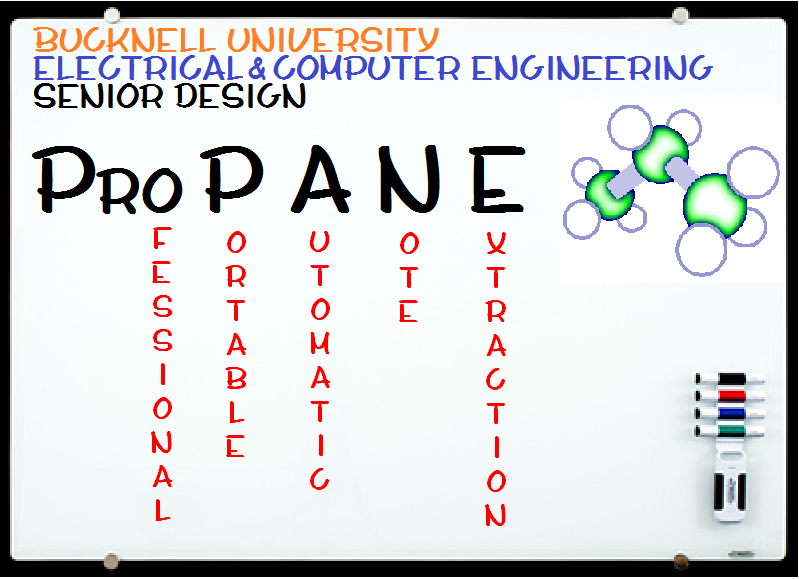
\includegraphics[scale=0.36]{images/propane_whiteboard}
\caption{Homepage image}
\end{figure}
 

	% Second Entry
	\section{Logo Design, Research on Background and Competition  (09/05/2012)}

		\subsection*{Logo Design}
		Worked on the ProPANE logo.  Tried different color schemes ranging anywhere from black and white, orange and blue (Bucknell) and black and gold.  Design was done in Adobe Photoshop and MS Paint.

\begin{figure}[H]
\begin{minipage}[b]{0.45\linewidth}
\centering
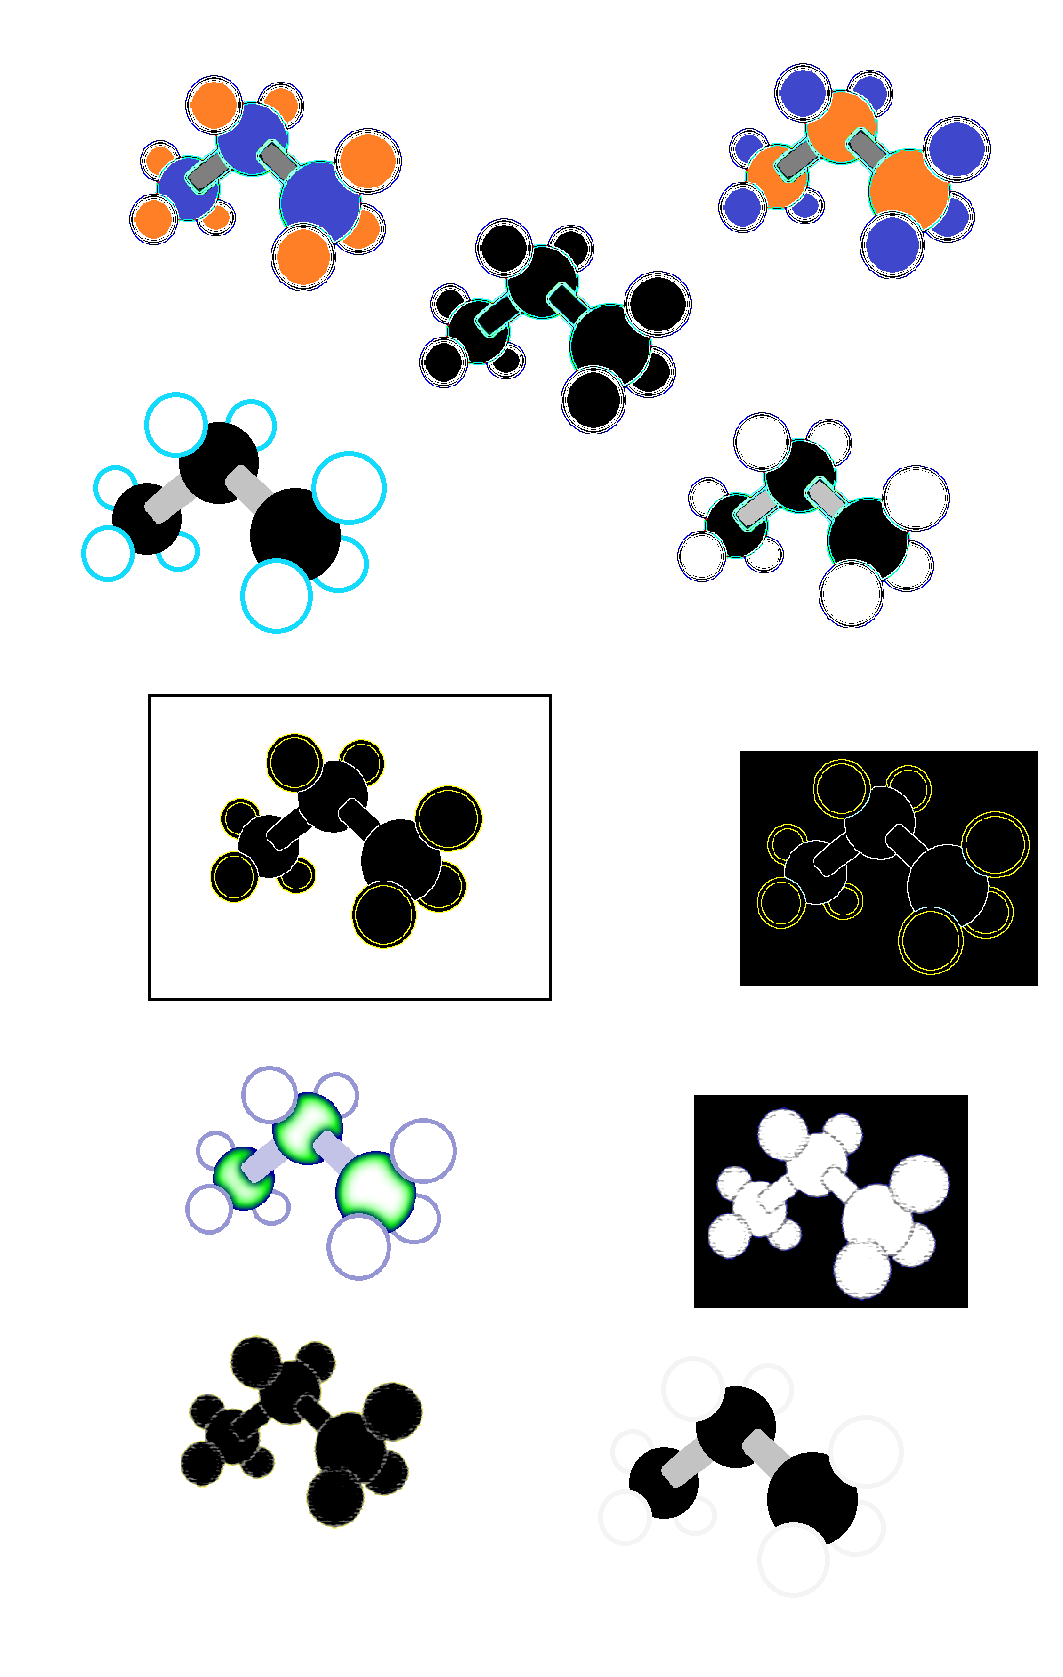
\includegraphics[scale=0.22]{images/logo_options}
\caption{Preliminary logo designs}
\end{minipage}
\begin{minipage}[b]{0.45\linewidth}
\centering
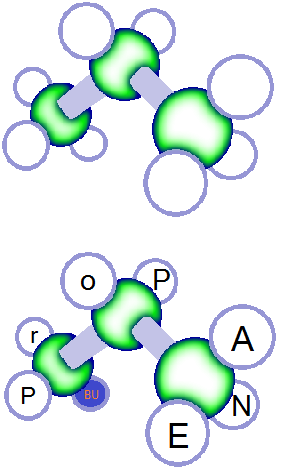
\includegraphics[scale=0.7]{images/ProPANE_final_logos}
\caption{Current ProPANE logos}
\end{minipage}
\end{figure}

Eventually the group settled on the current logos above, because they are easy on the eyes yet they still stand out.  \\

		\subsection*{Background Research}
			We began researching the different existing technologies that meet standards similar to that of our project.  One in particular seemed very similar to the design we are aiming for: a research project by Microsoft, their Whiteboard Capture System \href{ftp://ftp.research.microsoft.com/pub/tr/tr-2002-89.pdf}{(link)}.  I am in charge of analyzing it for inclusion in our Project Background and Research document.  

The Whiteboard Capture System is portable, works on any whiteboard, and provides a method of data distribution, all of which are desirable for our system.  However, it has some shortcomings (does not work on blackboards) and possible excess features (audio recording and playback).  Full  analysis will be included in the final document.    \\
			
			
			
	
	% First Entry
	\section{First Group Meeting and General Group Information  (08/31/2012)}
		
		Talked about the Initial Group Tasks.  Came up with a name, logo, and document template.  Discussed general tech specs and background information.    
		
		\subsection*{Technical Specifications}
			Our end design must be a portable system which captures notes written on a chalkboard or whiteboard, and distributes the information for later use.  We are looking into similar products which are currently on the market for background info and implementation ideas.  Dr. Midkiff plans to use our system to aid students with disabilities, so extra attention must be paid to ease of use and clarity of the final deliverable product.      \\
		
		\subsection*{Team Name and Logo}
			We wated to come up with an acronym that was both relevant to our project in some way, and also easy to say. We settled on the name BU ProPANE, which stands for \textbf{Pro}fessional \textbf{P}ortable \textbf{A}utomatic \textbf{N}ote  \textbf{E}xtraction.  We liked the idea of an already well-known word for the name, and we decided to design a logo with the same theme.  I am currently working with an image of a propane molecule to design a logo for BU ProPANE.    \\
			
		\subsection*{Document Template}
			We are using \LaTeX to format our documents and deliverables.  It was chosen because it takes care of formatting for us.   \\
			

\end{document}